\documentclass[12pt]{article}
\usepackage{graphicx}
\usepackage{amsmath}

\begin{document}
\begin{titlepage}
	\begin{center}
	\line(1,0){300}\\
	[0.25in]
	\huge{\bfseries Lab 1: Kinematic Characterization of the Lynx (MATLAB)}\\
	[0.12in]
	\line(1,0){200}\\
	[1cm]
	\textsc{\Large University of Pennsylvania}\\
	\end{center}
	\vfill
	\begin{flushright}
	\textsc{\large Wesley Yee, Shaun Fedrick\\
	MEAM 520\\
	September 23, 2020\\}
	\end{flushright}
\end{titlepage}

\begin{enumerate}
\item \begin{figure}
	\centering 
	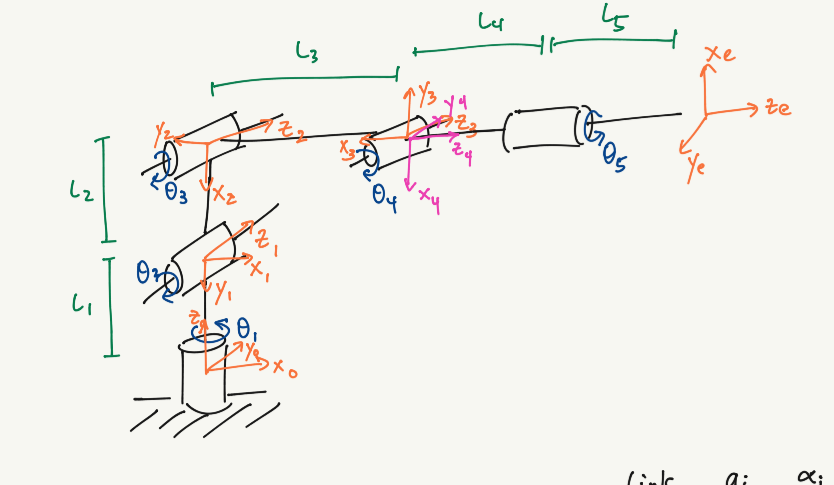
\includegraphics[scale=1]{Q1.png}
	\caption{Revised symbolic representation}
	\end{figure}
\item 
\begin{equation}
	T^{0}_{1} = \begin{bmatrix}
	0 & 0 & 1 & 0mm\\
	-1 & 0 & 0 & 0mm\\
	0 & -1 & 0 & 76.2mm\\
	0 & 0 & 0 & 1
	\end{bmatrix}
\end{equation}

\begin{equation}	
	T^{1}_{2} = \begin{bmatrix}
	0 & -1 & 1 & 0mm\\
	1 & 0 & 0 & 146.05mm\\
	0 & 0 & 1 & 0mm\\
	0 & 0 & 0 & 1
	\end{bmatrix}
\end{equation}

\begin{equation}	
	T^{2}_{3} = \begin{bmatrix}
	-\frac{\sqrt{2}}{2} & -\frac{\sqrt{2}}{2} & 0 & -132.4588mm\\
	\frac{\sqrt{2}}{2} & -\frac{\sqrt{2}}{2} & 0 & 132.4588mm\\
	0 & 0 & 1 & 0mm\\
	0 & 0 & 0 & 1
	\end{bmatrix}
\end{equation}

\begin{equation}	
	T^{3}_{4} = \begin{bmatrix}
	0 & 0 & -1 & 0mm\\
	-1 & 0 & 0 & 132.4588mm\\
	0 & 1 & 0 & 0mm\\
	0 & 0 & 0 & 1
	\end{bmatrix}
\end{equation}

\begin{equation}	
	T^{4}_{5} = \begin{bmatrix}
	0 & 1 & 0 & 0mm\\
	-1 & 0 & 0 & 0mm\\
	0 & 0 & 1 & 68mm\\
	0 & 0 & 0 & 1
	\end{bmatrix}
\end{equation}

\begin{equation}	
	T^{4}_{5} = \begin{bmatrix}
	-1 & 0 & 0 & 0mm\\
	0 & \frac{\sqrt{2}}{2} & -\frac{\sqrt{2}}{2} & 84.3755mm\\
	0 & -\frac{\sqrt{2}}{2} & -\frac{\sqrt{2}}{2} & 14.5255mm\\
	0 & 0 & 0 & 1
	\end{bmatrix}
\end{equation}
\item 
\item 
\end{enumerate}

\end{document}
